One of the most used patterns in parallel computing is the reduction. The reduction combines all elements in an array to a single element using an reduction operator. This can for example be used to calculate the sum or product of an array. In order for the reduction to happen the reduction operator must be both binary and associative. Binary means that the operator is two-to-one, combining two element to one. Associative means that the order of which operations are performed does not effect the result. So for any operator $\oplus$ \cref{eq:al_associative} must hold.

\begin{equation} 
\label{eq:al_associative}
	(a \oplus b) \oplus c = a \oplus (b \oplus c)
\end{equation}



\begin{figure}[ht]
	\centering
	\fbox{
		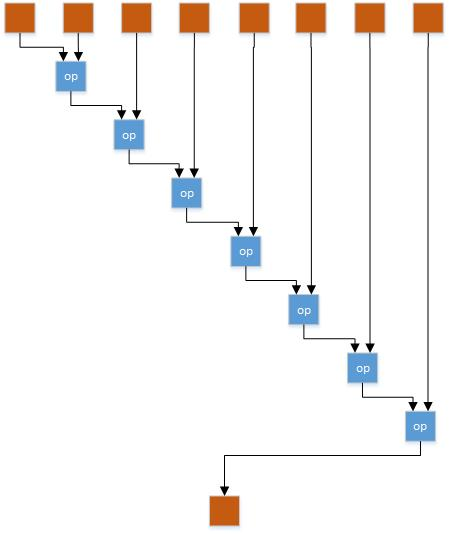
\includegraphics[width=0.6\textwidth]{figs/algorithm/reduce_serial.jpg}}
	\caption{TBD}
	\label{fig:reduce_serial}
\end{figure}



\begin{figure}[ht]
	\centering
	\fbox{
		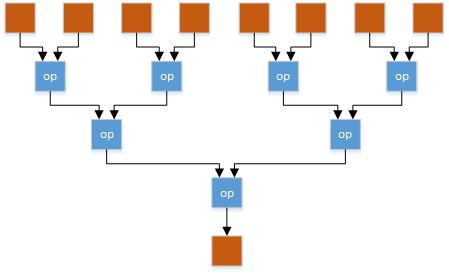
\includegraphics[width=0.6\textwidth]{figs/algorithm/reduce_parallel.jpg}}
	\caption{TBD}
	\label{fig:reduce_parallel}
\end{figure}


\begin{figure}[ht]
	\centering
	\fbox{
		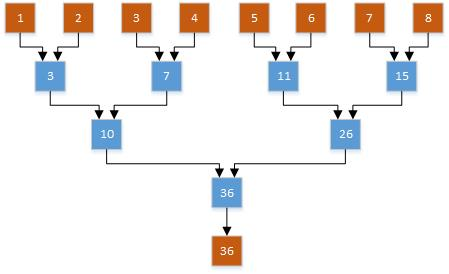
\includegraphics[width=0.6\textwidth]{figs/algorithm/reduce_parallel_example.jpg}}
	\caption{TBD}
	\label{fig:reduce_parallel_example}
\end{figure}
